\documentclass[a4paper,twoside,11pt]{article}
\usepackage[utf8]{inputenc}
\usepackage{graphicx}
\usepackage{graphics}
\usepackage{amsmath,amsfonts,amssymb}
\usepackage{float}
\usepackage{placeins} %met des barrières aux floats
\usepackage{color} %pour changer la couler du texte
\usepackage{cases}
\usepackage{cite}
\usepackage{multirow}
\usepackage{setspace} % pour changer l'interligne poncutellement

%math operator, text style in equations
\DeclareMathOperator{\im}{i} %nombre imaginaire
\DeclareMathOperator{\e}{e} %nombre exponentiel
\DeclareMathOperator{\inc}{inc}
\DeclareMathOperator{\R}{R}
\DeclareMathOperator{\T}{T}
\allowdisplaybreaks %pour permettre de couper une equation pour qu'elle tienne 
%sur plusieurs pages

\usepackage[top=2.5cm,bottom=2cm,inner=2.5cm,outer=1.5cm]{geometry} 

%========>>> Style des légendes
\makeatletter
\renewcommand{\fnum@table}{\small\textbf{Tableau~\thetable}}
\renewcommand{\fnum@figure}{\small\textbf{Figure~\thefigure}}
\makeatother

\makeindex

\title{\large{Introduction to acoustic imaging}}

\author{\large{echOpen CC BY-SA}}

\begin{document}
%\begin{titlepage}
\thispagestyle{empty}
%\setlength{\baselineskip}{0.8\baselineskip}

%\voffset 0,6cm
%\hoffset -30.5mm
\noindent

\vspace*{0.6cm}

\begin{center}
{\bf\huge }
\noindent\vspace*{0,5cm}

{}
\noindent\vspace*{0,5cm}

{\bf\huge }
\noindent\vspace*{0,5cm}


\noindent\vspace*{1cm}


\noindent\vspace*{1cm}

\begin{figure}[htb]
  \centering
		
\includegraphics[width=0.2\textwidth]{image/logo}
\end{figure}
\noindent\vspace*{0,5cm}


\noindent\vspace*{0,5cm}


\noindent\vspace*{1cm}

{\bf --------}
\noindent\vspace*{0.2cm}

{\bf \Huge Introduction to acoustic imaging}
\noindent\vspace*{0,2cm}

{\bf --------}
\noindent\vspace*{0,9cm}
\end{center}

\noindent

\vspace*{0.4cm}

\noindent

\noindent\vspace*{0.4cm}
%{\bf\Large echOpen}
\noindent


\vspace*{0.4cm}

\noindent
%{\bf\Large CC BY-SA}
\noindent\vspace*{0,5cm}
\begin{figure}[htb]
  \centering
		
\includegraphics[width=0.2\textwidth]{image/license}
\end{figure}
\noindent


%\vfill


%\newpage



%\end{titlepage}
\clearpage

\tableofcontents
\clearpage

In this document, we will explain some basis of the acoustic theory to 
understand the propagation of acoustic waves and the echographic process.

\section{Propagation of acoustic waves}
\label{sec:Propagation of acoustic waves}

In this section, we will define the different types of acoustic waves and some 
basic equations and properties of the propagation of acoustic waves.

\subsection{Wave types}
\label{sec:wave types}

\FloatBarrier

An acoustic wave is a perturbation of the local state without displacement of 
the global state. Acoustic waves are periodic, their spatial periodicity is 
given by the wavelength $\lambda$. Consider a medium at rest such as on 
Fig.~\ref{fig:at_rest}, where the particles are represented by the dots. Such a 
periodic structure represent a metal for example. When an acoustic wave 
propagate in this medium, the particles will have a local displacement.

\begin{figure}[htb]
	\centering
		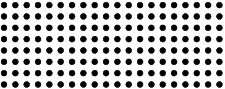
\includegraphics{image/at_rest}
	\caption{Medium at rest.}
	\label{fig:at_rest}
\end{figure}

There is two types of acoustic waves, the longitudinal waves 
(Fig.~\ref{fig:Pwave}) also named P waves and the transverse 
waves (Fig.~\ref{fig:Swave}) also named SH or SV waves. The longitudinal waves 
are compressional waves, the direction of the 
displacement of the particles is the same than the direction of propagation of 
the wave. The transverse waves are shear waves, the direction of displacement 
is then perpendicular to the direction of propagation of the wave. In a fluid, 
such as the water, only longitudinal waves can propagate. In the human body, 
the 
shear modulus is very small, it can be considered as a fluid, and so only 
longitudinal waves will be generated.

\begin{figure}[htb]
	\centering
		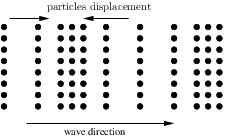
\includegraphics{image/Pwave}
	\caption{Longitudinal wave.}
	\label{fig:Pwave}
\end{figure}
\begin{figure}[htb]
	\centering
		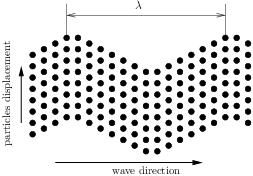
\includegraphics{image/Swave}
	\caption{Shear wave.}
	\label{fig:Swave}
\end{figure}

In the rest of the document, we will only consider longitudinal waves.

\FloatBarrier

\subsection{Mathematical formulation}
\label{sec/Mathematical formulation}

In acoustic, a fluid medium is describe by two mecanical parameters: the mass 
density 
$\rho$ and the bulk modulus $\kappa$. The bulk modulus relate the change of 
volume of a medium to the isostatic pressure apply on it. The velocity of the 
acoustic wave $c$ is:
\begin{equation}
 c=\sqrt{\dfrac{\kappa}{\rho}},
 \label{eq:speed of sound}
\end{equation}
for example, for the water we have: $\rho=1000\text{ kg.m}^{-3}$, 
$\kappa=2.19\text{ MPa}$ and $c=1480\text{ m.s}^{-1}$.

The mathematical formulation is obtained by solving the Helmholtz equation, for 
exemple, the acoustic pressure $p\left(x,t\right)$ can be expressed as:
\begin{equation}
 p\left(x,t\right)=\left(A^{+}\e^{\im kx}+A^{-}\e^{-\im kx}\right)\e^{-\im 
\omega t},
 \label{eq:math 1D formulation}
\end{equation}
$A^{+}\e^{\im kx}$ is a wave of amplitude $A^{+}$, propagating toward the 
positive $x$, $A^{-}\e^{-\im kx}$ is a wave of amplitude $A^{-}$, propagating 
toward the negative $x$. $k=\dfrac{\omega}{c}$ is the wavenumber, $\omega=2\pi 
f$ the angular pulsation and $f$ the frequency.

When we make an echographic image, we are intresting only on the intensity of 
the wave:
\begin{equation}
 I=\dfrac{1}{2}\Re\left[p\left(x,t\right)v^{*}\left(x,t\right)\right],
 \label{eq:acoustic intensity}
\end{equation}
where $v\left(x,t\right)$ is the velocity of the particle, and $x^{*}$ 
represent 
the complex conjugate of $x$. It can be shown with the Euler's equation that 
the 
intensity is directly proportional to the square modulus of the pressure.

\subsection{Refraction and diffusion of acoustic waves}
\label{sec:Refraction and diffusion of acoustic waves}

When an acoustic wave passes from a medium (0) to a second medium (1), a part 
of 
the wave is reflected an the over part is transmitted through the interface. 
When the interface is flat in the point of view of the wave, we have refraction 
(it is a quasi one dimensional problem, because the wave is reflected on 
only one direction of the space). When the wave sees the curvature of the 
interface, the wave is scattered on all the directions of the space, we talk 
then about diffusion.

\subsubsection{Refraction of a wave}
\label{sec:Refraction of a wave}

\begin{figure}[htb]
	\centering
		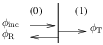
\includegraphics{image/refraction}
	\caption{Refraction of a wave.}
	\label{fig:refraction}
\end{figure}

We consider an incident wave $\phi_{\inc}$ normal to an interface, the reflected 
$\phi_{R}=R\phi_{\inc}$ and the transmitted $\phi_{T}=T\phi_{\inc}$ waves are 
also normal to the interface (Fig.~\ref{fig:refraction}). $R$ and $T$ represent 
respectively the reflexion and transmission coefficient. By solving this 
problem, we show that:
\begin{equation}
 R=\dfrac{Z_2-Z_1}{Z_2+Z_1},
 \label{eq:reflection coefficient}
\end{equation}
where $Z_i=\rho_ic_i$ is the acoustic impedance of the medium $i$.

If we consider, for example the reflection of a wave at an interface between 
water 
($\rho_0=1000\text{ kg.m}^{-3}$, $c_0=1480\text{ m.s}^{-1}$) and a muscle 
($\rho_1=1070\text{ kg.m}^{-3}$, $c_1=1590\text{ m.s}^{-1}$), the 
reflection coefficient is equal to $69.10^{-3}$, so only 7\% of the pressure is reflected. 
If we know consider an interface between water and bone ($\rho_1=2175\text{ 
kg.m}^{-3}$, $c_1=4000\text{ m.s}^{-1}$), then nearly 70\% of the incident wave 
is reflected. The echos due to bones are much more higher than the ones due to 
the muscles. 

\subsubsection{Scattering of a wave}
\label{sec:Diffusion of a wave}

Even if an object is very small in front of a wave, it always scattered the 
wave 
(Fig.~\ref{fig:diffusion}). It is much more complicated to determine the 
scattered wave than the reflected wave such as in sec.~\ref{sec:Refraction of a wave}.

\begin{figure}[htb]
	\centering
		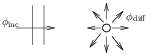
\includegraphics{image/diffusion}
	\caption{Scattering of a wave.}
	\label{fig:diffusion}
\end{figure}

The diffused wave goes in every direction of the space, it lead that its 
amplitude 
decreases with the distance from the object.

\subsection{Attenuative media}
\label{sec:Attenuative media}

The human body is an attenuative media, this mean that the amplitude of a wave 
propagating in such medium decreases along its direction of propagation. 
Mathematically, the propagation of waves in this kind of medium is written as:
\begin{equation}
 p\left(x,t\right)=\left(A^{+}\e^{\im kx}\e^{-\alpha x}+A^{-}\e^{-\im 
kx}\e^{\alpha x}\right)\e^{-\im 
\omega t}.
 \label{eq:math 1D absobing formulation}
\end{equation}
The difference between the propagation of a wave between a non-attenuative and 
an attenuative medium is present on Fig.~\ref{fig:attenuative medium}. So when 
we do acoustic imaging in the human body, we must gradually amplify the 
received signal if we want to convert correctly the analogical signal into a 
digital signal, because if the amplitude of the signal is smaller than the precision 
of the ADC, we can't measure it (see appendix~\ref{sec:ADC}). Classically, we 
do Time Gain Compensation (TGC) on the receive signal in order to keep a 
convenient amplitude of the received signal. An example of this kind of 
treatment is presented on Fig.~\ref{fig:tgc example}, it's apply to the 
attenuated signal on the right side of Fig.~\ref{fig:attenuative medium}.

\begin{figure}[htb]
	\centering
		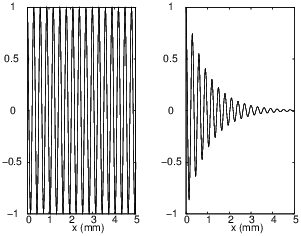
\includegraphics{image/attenuative_medium}
	\caption{Acoustic pressure of a wave propagating in a non-attenuative 
(left) and attenuative (right) medium.}
	\label{fig:attenuative medium}
\end{figure}

\begin{figure}[htb]
	\centering
		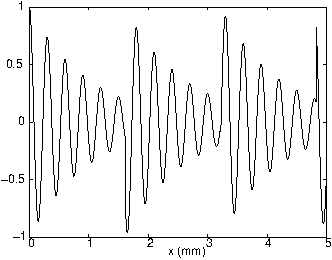
\includegraphics{image/tgc_example}
	\caption{Example of TGC applied on the attenuated signal (right side of 
Fig.~\ref{fig:attenuative medium}.}
	\label{fig:tgc example}
\end{figure}



\clearpage
\section{Transducer}
\label{sec:Transducer}

A transducer is an acoustic sensor, it convert electric power to mechanical 
power and conversely. So if you apply an electric signal on it, it will 
generate acoustic wave (like a speaker), and if an acoustic wave deform it, it 
generate an electrical signal (like a microphone).

In order to have a correct radial precision in acoustic imaging, the acoustic 
wave must be focused on one point. This can be done by two kind of technologies: 
focussed transducer and transducers array.

\subsection{Focussed transducer}
\label{sec:Focussed transducer}

\begin{figure}[htb]
	\centering
		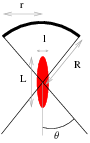
\includegraphics{image/transducer_scheme}
	\caption{Acoustic wave focalisation (red) by a focussed transducer.}
	\label{fig:transducer scheme}
\end{figure}

This kind of transducer have a spherical shape, so the emitted acoustic wave 
naturally focalised at the center of the sphere (Fig.~\ref{fig:transducer 
scheme}). The area of the focal spot is an ellipse, the value of $l$ and $L$ can 
be approximate by:
\begin{equation}
 l=\dfrac{\lambda R}{2r},
 \label{eq:l value}
\end{equation}
\begin{equation}
 L=15\left(1-0.01\theta\right)l.
 \label{eq:L value}
\end{equation}
More $\theta$ is high, more the ellipse is small. When we do acoustic imaging, 
we want $l$ to be as small as possible to increase the radial precision. 
Moreover we want $L$ to be high, because the echo of an object outside of this 
ellipse will be too small to be measured. So we have to make a compromise between 
$l$ and $L$.

At the nearfield (it depend on $\lambda$ and $r$) of the transducer, the 
acoustic pressure is to chaotic so we can't do acoustic imaging in the 
nearfield of this kind of transducer.

\subsection{Transducers array}
\label{sec:Transducers array}

On a transducers array, generally, the size of each transducer is small compare 
to the wavelength, so they emit spherical waves. If all the transducers emit a 
wave at the same time, the array will emit a plan wave. If you apply a right 
delay between the emission of each transducer it is possible to generate a 
focussed acoustic wave (Fig.~\ref{fig:transducers array}). This delay can be 
simply calculated, indeed, by knowing the distance between each transducer, you 
just have to determine a delay that consist on having all the wave generated by 
each transducer arriving exactly at the same on a given point of the space. By 
doing this the waves interfere coherently near this point (high pressure) and 
incoherently everywhere else (low pressure).


\begin{figure}[htb]
	\centering
		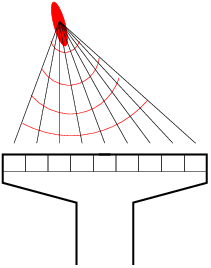
\includegraphics[width=0.3\textwidth]{image/transducers_array}
	\caption{Acoustic wave focalisation with an array of transducers.}
	\label{fig:transducers array}
\end{figure}

With a transducers array, it is possible to focalise at different points at the 
same time, so acoustic imaging can be faster with this and it don't need a motor to 
image a plane. However they are much more expensive than a simple focussed 
transducer and the electronic is much more complicated to drive a transducers 
array. 

\clearpage
\section{Signal Processing}
\label{sec:Signal Processing}

In this section we introduce the Fast Fourier Transform (FFT) and present a 
basic signal processing to improve an echographic signal.

\subsection{Fast Fourier Transform}
\label{sec:Fast Fourier Transform}
\FloatBarrier

The Fourier Transform is a transformation that express a function of a given 
dimension as a function of another dimension. Classically, a time dependent 
signal is expressed as a function of the frequencies. In acoustic we also apply 
Fourier transform to a space signal, so the transform is a function of the 
wavelength. The Fourier Transform $S$ of a real signal $s$ is complex and 
$\Re\left(S\right)$ is an even function and $\Im\left(S\right)$ is odd.

The FFT is an algorithm that calculate the Fourier Transform of a signal very 
fast, the number of point of the signal must be a power of 2. The FFT of a signal 
is a periodic function with a periodicity equal to the frequency sampling of the 
initial signal. Classically, the FFT algorithm return the Fourier Transform for 
the positive frequencies. Due to the periodicity of the FFT, the second half of 
the signal is the negative frequency part.

Consider a time signal sample at frequency $f_e=640$ MHz composed of N=1024 
points (Fig.~\ref{fig:time signal}). If you keep only the positive frequencies, 
the frequency vector corresponding to the FFT go from 0 to $f_e\dfrac{N-1}{N}$. 
On octave its given by linspace(0,fe*(N-1)/N,N). The FFT of the time signal 
keeping the positive frequencies is presented on Fig.~\ref{fig:positive 
frequencies}.

If one want to filter the signal, it is more convenient to consider the 
negative frequencies, because if you want to filter the a signal between x and y 
MHz, you must put to 0 all frequencies except the points between x and y MHz 
and also the points between -x and -y MHz. In this case, the frequency vector 
is given by linspace(-fe/2*(N-1)/Nfe/2,N) and you must put the second half of 
the FFT signal at the beginning. To do that you must create a new vector of the 
same size than the FFT signal, and doing fox example: S2(1:N/2-1)=S(N/2+2:end) 
and S2(N/2:end)=S(1:N/2+1). Then you obtain the signal presented on 
Fig.~\ref{fig:negative frequencies}.

The real and imaginary part of the FFT presented on Figs.~\ref{fig:positive 
frequencies} and \ref{fig:negative frequencies} are divided by their maximum 
amplitude to have readable graphics.

If one want to know the central frequency of a transducer, you must take the 
modulus of the FFT of an echo of the transducer. The central frequency is the 
frequency where the modulus has the higher value.

\begin{figure}[htb]
	\centering
		\includegraphics{image/time_signalb}
	\caption{Example of a time signal.}
	\label{fig:time signal}
\end{figure}
\begin{figure}[htb]
	\centering
		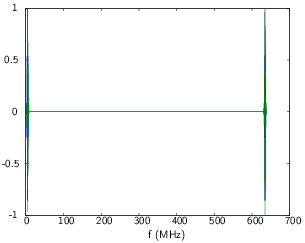
\includegraphics{image/positive_frequenciesb}
	\caption{FFT of the signal presented on Fig.~\ref{fig:time signal} 
keeping the positive frequencies. On blue real part and green imaginary part.}
	\label{fig:positive frequencies}
\end{figure}
\begin{figure}[htb]
	\centering
		\includegraphics{image/negative_frequenciesb}
	\caption{FFT of the signal presented on Fig.~\ref{fig:time signal} with 
the negative frequencies. On blue real part and green imaginary part.}
	\label{fig:negative frequencies}
\end{figure}

\FloatBarrier
\subsection{Hilbert transform}
\label{sec:Hilbert transform}

The Hilbert transform is useful for signal processing in echographic imaging, 
because with this transformation we can access to the envelop of a given 
signal. The Hilbert transform can be determine easily with the FFT. Indeed, if 
you calculate the FFT of a signal and put all the negative frequencies to 0 and 
do an IFFT (Inverse Fast Fourier Transform), then you have the Hilbert 
transform of the signal. By doing this to the signal presented in 
Fig.~\ref{fig:time signal}, we obtain the transform signal presented on 
Fig.~\ref{fig:hilbert transform}. 

\begin{figure}[htb]
	\centering
		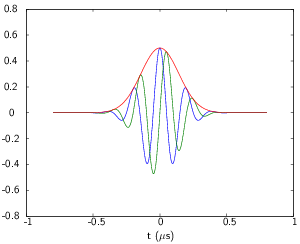
\includegraphics{image/hilbert_transformb}
	\caption{Hilbert transform of the signal presented on 
Fig.~\ref{fig:time signal}. Blue real part, green imaginary part and red 
modulus.}
	\label{fig:hilbert transform}
\end{figure}

\subsection{Basic echographic signal processing}
\label{sec:Basic echographic signal processing}

The most basic signal processing for echographic imaging is to filter the 
signal and extract the envelop of the filtered signal. So you make a FFT of 
the signal measured by the transducer and you filter $\pm$ 2 MHz around the 
central frequency of the transducer for example, lets say between 5.5 and 9.5 
MHz for a transducer centered at 7.5 MHz. You can keep the positive frequency, 
so you put all frequency smaller than 5.5 and higher than 9.5 MHz to 0. By 
doing this you apply a square window on the signal, you can also apply an 
Hamming, Hanning or Blackmann window. The negative frequency are also put to 0 
with this method so if you make an IFFT, you apply a Hilbert transform to the 
filtered signal. By taking the modulus so we access to the envelop of the 
filtered signal.

Now we have to define the pixels of the image. For example we can say that a 
pixel as the same length that the wavelength $\lambda$ of the acoustic wave, 
$\lambda=\dfrac{c}{f}$ ($c$ = 1500 m.s$^{-1}$). The time $t$ needed to 
travelled a distance $d$ is $t=\dfrac{2d}{c}$ (2 because the wave travelled 
back and forth) so if $d = \lambda$ then $t = 26.7 \mu$s. At 640 MHz, it 
correspond to 171 time points. The value of pixel is then define by integrated 
the signal on 171 points. An echographic image show the value of the acoustic 
power in dB, so to obtain this you just have to plot $20\log\left(s\right)$. 
Where $s$ is the envelop of the filtered signal integrated on the adequate 
number of time points.

\clearpage
\addcontentsline{toc}{part}{Annexes}

\part*{Annexes}

\label{sec:Annexes}



\appendix

\section{ADC}
\label{sec:ADC}

In this appendix, we make a quick introduction to Analogical Digital Converter. 
This component is one of the most important in an echographic probe, so it is 
necessary to understand how does it work.

As its name suggest, an ADC convert the algebrical value of the tension of a 
signal to a digital signal. To remember, a digital signal is a binary signal, 
the 0 correspond to 0 V, the low value and 1 correspond to high 
value (5 V for example). In a computer or smartphone, all the treatment are 
made in the digital form, so it is necessary to convert the analogical signal 
measured on the transducer to a digital signal. An ADC is characterized by its 
sampling rate expressed in sampling per second (Sps) and its precision $n$. The 
sampling rate define the number of time it convert a signal per second. The 
precision define on how many bites the digital number is written, so the ADC 
sample the signal on $2^n$ values.

An ADC is supply with a given continuous current $V_{\text{cc}}$. So the ADC 
sampling of the analogical are $2^n$ value equally space between 
$-V_{\text{cc}}$ (or 0V) and $+V_{\text{cc}}$. The precision $p$ of the ADC is 
then:
\begin{equation}
 p=\dfrac{2V_{\text{cc}}}{2^n-1}.
 \label{eq:precision adc}
\end{equation}
So if we have $V_{\text{cc}}=5$ V on a 8 bites ADC ($n=8$), then the precision 
is then 39.2 mV. Now consider than the output $k$ of the ADC is an unsigned 
integer (this mean that the output is 0 to 255) then the voltage $V_{\text{m}}$ 
of the analogical signal is:
\begin{equation}
 V_{\text{m}}=-V_{\text{cc}}+kp,
 \label{eq:voltage value adc}
\end{equation}
so if $k=23$ then the analogical signal is -4.1 V high.




\end{document}
